\chapter{Proof of concept d'une attaque}
\label{chap:attaque}

L'implémentation de \og \gls{safeStack} \fg au sein de \gls{llvm} doit permettre de prévenir les attaques se basant sur l'exploitation d'un dépassement de tampon. Dans ce chapitre un \og proof of concept \fg d'une telle attaque est décrit sur un exemple de code fictif. Afin de rendre plus portable et reproductible cette phase de test, un environnement spécifique est mis en place et décrit précisément ainsi que la recette utilisée lors de la phase de compilation.

L'objectif est de démontrer l'efficacité de \gls{levee} et de comparer l'approche avec celle des \og \gls{stackCookies} \fg. Pour ce faire, une première attaque a été pensée, malheureusement celle-ci n'avais pas la possibilité d'aboutir. Basée sur ces conclusions, une autre attaque a été mise en place. Leur descriptions théorique ainsi que leurs implémentations sont décrites dans ce chapitre.

Un des exemples d'attaque proposé dans ce chapitre est basé sur l'article \og Introduction to return oriented programming (ROP) \fg du blog \textit{codearcana.com} \cite{IntroductionToROP}.

\minitoc

\newpage

% -----------------------------------------------------------------------------
\section{Environnement}

Afin de faciliter la mise en place de l'attaque, la compilation est faite en 32~bits. L'environnement choisi pour installer la version 4.0 de \gls{llvm} est Debian 8 en 64~bits. Afin de pouvoir correctement compiler et exécuter en 32~bits, les bibliothèques nécessaires doivent être installées (lignes 20 à 22). En plus de \gls{llvm}, \gls{gdb} ainsi que quelques autres utilitaires sont installés.

\subsection{Docker}

L'environnement décrit ci-dessus ainsi que l'installation des outils sont mis en place grâce à Docker. Le Dockerfile suivant contient toutes les instructions nécessaires afin d'installer la version 4.0 de \gls{llvm} et \gls{clang}.

\begin{listing}
	\dockerfile{02-main/listings/Dockerfile}
	\caption{Fichier décrivant l'environnement choisi pour l'installation de \gls{llvm} 4 sous Debian 8}
	\label{lst:dockerfile}
\end{listing}

Il existe plusieurs manières d'installer \gls{llvm}. Il serait tout à fait possible de compiler directement depuis les sources. Plusieurs de ces techniques ont été testées, et la suivante a été retenue: l'installation de Clang 4.0, \gls{lldb} (équivalant de \gls{gdb}) et de LLD (le \og linker \fg de \gls{llvm}) se fait en rajoutant le dépôt APT de \gls{llvm}. Après plusieurs essais, le débogueur \gls{gdb} est préféré à \gls{lldb} et est par la suite utilisé à la place de \gls{lldb}, ce dernier n'étant pas encore assez complet et globalement utilisé.

Tout les autres fichiers de configurations de l'environnement Docker sont disponibles à l'annexe \ref{chap:dockerConf}.

\subsection{Gestion de la compilation}

L'utilitaire \textit{make} est utilisé pour gérer le processus de compilation. Un Makefile est mis en place afin de rassembler les différents \og flags \fg utilisés pour générer les deux versions exécutables (l'un avec \gls{safeStack} et l'autre sans). En en-tête, différentes variables utilisées par \textit{make} sont définies afin de s'assurer que \gls{clang} 4.0 est bien utilisé. Deux version de l'exécutable sont créés: \textit{safe-stack} et \textit{stack-cookie}. Le language intermédiaire de \gls{llvm} est émis lors de la compilation afin de comparer les effets de l'un et l'autre mécanisme de protection.

À noter que la protection de la pile \texttt{\textit{-fstack-protector}} est desactivée grâce à \texttt{\textit{-fno-stack-protector}} lorsque l'on active \og \gls{safeStack} \fg. Le but étant de comparer les deux mécanismes, qui plus est, actuellement \og \gls{safeStack} \fg n'est pas compatible avec les \og \gls{stackCookies} \fg.

\begin{listing}
	\makefile{02-main/listings/Makefile}
	\caption{Makefile regroupant les différentes options de compilations}
	\label{lst:defaultMakefile}
\end{listing}

Un script permettant d'afficher les mécanismes de protection d'un binaire est utilisé, pour cela une règle spécifique aux tests est décrite à la ligne 38.

\vfill

\subsection{Mécanismes de sécurité actifs}

\gls{aslr} est actif au sein de l'environnement. Chaque binaire est protégé soit avec \og \gls{stackCookies} \fg ou avec \og \gls{safeStack} \fg. Le script \mintinline{bash}{checksec.sh} \cite{CheckSec} est utilisé pour afficher les mécanismes actifs sur chaque binaire. On peut constater sur le résultat ci-dessous que les \og \gls{stackCookies} \fg sont bien désactivés lors du test de \og \gls{safeStack} \fg et que dans les deux cas le drapeau \gls{nx} est actif.

\begin{listing}
	\bashfile{02-main/listings/checksec.res}
	\caption{Resultat du test de sécurité par checksec.sh}
	\label{lst:checksecRes}
\end{listing}

\gls{pie} est un mécanisme de protection récent qui permet d'appliquer de l'aléatoire sur des régions de code, et ainsi rendre plus difficile la mise en place d'une attque de type \gls{rop}.


% -----------------------------------------------------------------------------
\section{Pointeur de fonction sur la pile}

\subsection{Description théorique de l'attaque}

La première tentative se base sur une \textit{structure} dans laquelle est stocké un pointeur vers une fonction. En plaçant la \textit{structure} et le tampon sur la pile d'exécution, l'idée est de réécrire l'adresse du pointeur présent dans ladite \textit{structure} afin de lancer la chaîne de gadgets à l'appel du pointeur.

Le but est de mettre en place une \og stack frame \fg correspondant à la fonction \mintinline{c}{main()} ayant les variables locales stockées dans l'ordre dans lesquelles elles sont déclarées, comme le montre la \autoref{fig:attackStructExpected}.

\begin{figure}[H]
	\centering
	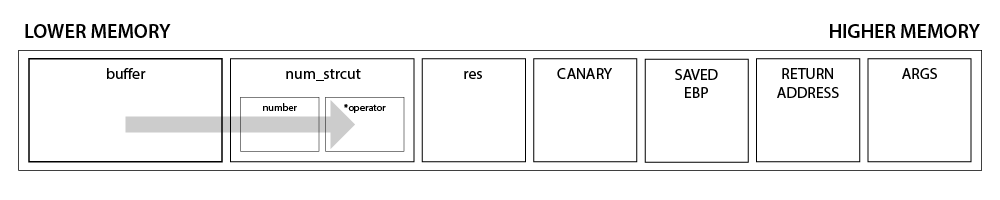
\includegraphics[width=1\columnwidth]{attackStructExpected}
	\captionsource{Résultat attendu de la \og stack frame \fg sur la première attaque}
	{Résultat attendu de la \og stack frame \fg sur la première attaque}
	{Auteur}
	\label{fig:attackStructExpected}
\end{figure}

\subsection{Implémentation}

Le code correspondant au scénario, présenté en \autoref{lst:struct}, comprend: (i) une structure nommée \texttt{Number}, (ii) une fonction \texttt{call()} permettant d'appliquer la fonction pointée par la structure et (iii) une fonction retournant le carré --- très mal optimisé --- de la valeur passée en paramètre. La fonction \texttt{main()} initialise la structure sur la pile ainsi que le \texttt{buffer}, puis copie dans le buffer l'argument \texttt{argv[1]} passé à l'exécution et appelle la fonction \texttt{call()}. De manière théorique il est alors possible, via l'argument \texttt{argv[1]}, de réécrire l'adresse stockée dans la structure.

\begin{listing}
	\cfile{02-main/listings/struct.c}
	\caption{Source du premier scénario d'attaque}
	\label{lst:struct}
\end{listing}

Cependant, lorsque l'on inspecte la pile d'exécution, on se rend compte que l'ordre dans lequel les variables sont stockées a été modifié. Le \og buffer \fg est positionné en premier --- vers la gauche ---, ce qui rend impossible son exploitation. Ce comportement inattendu est le résultat d'une manipulation souhaitée par le compilateur. Afin de se prémunir au mieux contre l'exploitation des dépassements de tampon, il place les variables de type \mintinline{c}{char*} dans les adresses les plus hautes, juste après le canari. De cette manière, si un dépassement apparaît, il est tout de suite détecté par le canari.

\begin{figure}[H]
	\centering
	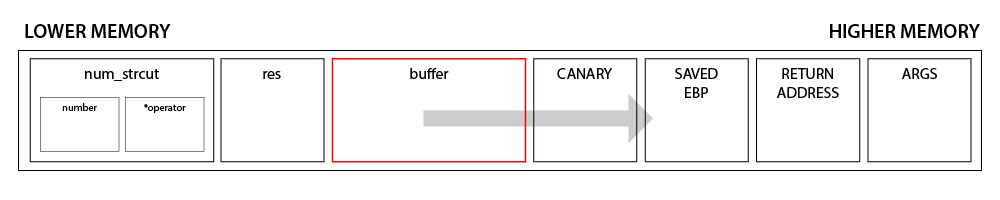
\includegraphics[width=1\columnwidth]{attackStructReel}
	\captionsource{Résultat obtenu de la \og stack frame \fg sur la première attaque}
	{Résultat obtenu de la \og stack frame \fg sur la première attaque}
	{Auteur}
	\label{fig:attackStructReel}
\end{figure}

\subsection{Conclusion}

Cette attaque ne peux pas aboutir et est détectée avec les deux mécanismes de protection. Le but ici est de démontrer les cas de figures où \og \gls{safeStack} \fg permet de se protéger contre des attaques qui ne seraient pas gardée par les \og \gls{stackCookies} \fg, cette attaque est donc abandonée au profit d'une nouvelle approche.


% -----------------------------------------------------------------------------
\section{Bypass du canari}

\subsection{Description théorique de l'attaque}
\subsection{Implémentation}
\subsection{Conclusion}


% -----------------------------------------------------------------------------
\section{Conclusions}
